%
% hydrodynamik.texo
%
% (c) 2018 Prof Dr Andreas Müller, Hochschule Rapperswil
%
\section{Fluiddynamik}
\rhead{Fluiddynamik}
%Die Atmosphäre und die Ozeane unterschieden sich in ihren
%für das Studium von Wetter und Klima wesentlichen Eigenschaften
%ganz beträchtlich.
%Das Wasser der Ozeane ist fast inkompressibel, seine Dichte hängt aber
%von der Temperatur und dem Salzgehalt ab.
%Wasser hat eine sehr grosse Wärmekapazität, ausserdem kann Wärme durch
%Verdunstung aus den Ozeanen in die Atmosphäre übergehen, wobei gleichzeigit
%die Salzkonzentration steigt.
%
%Die Atmosphäre auf der anderen Seite hat eine wesentlich geringere
%Dichte und Wärmekapazität, ihre Temperatur kann sich daher sehr viel
%schneller ändern.
%Sie ist stark kompressibel.
%Wegen der geringeren Dichte kann die Atmosphäre sehr viel höhere
%Strömungsgeschwindigkeiten erreichen.
%
%Trotz dieser grossen Unterschiede lassen sich Atmosphäre und Ozeane
%beide als Fluide mit den gleichen partiellen Differentialgleichungen
%beschreiben, die im folgenden hergeleitet werden sollen.
%Die Unterschiede äussern sich vor allem in den Zustandsgleichungen,
%die die Zustandsgrössen Druck, Temepratur, Dichte und Saltzgehalt
%miteinander in Beziehung setzen.
%
In diesem Abschnitt gehen wir davon aus, dass das Fluid beschrieben wird
durch Funktionen der Raumkoordinaten $(x,y,z)$ und der Zeit $t$,
wobei wir meistens darauf verzichten, die unabhängigen Variablen
auszuschreiben.
Die Temperatur $T$ ist also zu lesen als die Funktion $T(x,y,z,t)$.
Die Newtonschen Bewegungsgleichungen stellen eine Verbindung zwischen
Masse, Beschleunigung und Kraft her, wir können daher davon ausgehen,
dass die Bewegungsgleichungen eines Fluides nur die Dichte $\varrho$ und 
den Geschwindigkeitsvektor $\vec{v}$ involvieren.
Den Zusammenhang zwischen Druck, Temperatur, Dichte und möglicherweise
weiteren Eigenschaften wird durch Zustandsgleichungen vermittelt.

\subsection{Kontinuitätsgleichung}
Die Kontinuitätsgleichung drückt aus, dass
Materie nicht einfach neu entstehen oder verschwinden kann.
Um sie herzuleiten, betrachten wir ein Volumen $V$ des Fluids.
Die Masse im Inneren des Volumens wird bestimmt durch das Volumenintegral
\[
m
=
\iiint_V \varrho \,dx\,dy\,dz.
\]
Ein kleiner Quader mit den Abmessungen $\Delta x$, $\Delta y$
und $\Delta z$ enthält die Masse 
\[
m = \varrho \Delta x \,\Delta y \, \Delta z.
\]
Wenn sich die Masse in dem Quader ändert, dann muss Materie durch die
Wände zu- oder abfliessen.
Wir berechnen daher für jede Wand des Quaders, wie gross der Massefluss
durch die Wand in einer Zeiteinheit $\Delta t$ ist.

Durch ein Rechteck mit Abmessungen $\Delta y \times \Delta z$ senkrecht
zur $x$-Achse fliesst in der Zeit $\Delta t$ das Volumen
$v_x\Delta x\,\Delta y\,\Delta z$ und damit die Masse
\begin{equation}
\varrho v_x\,\Delta y\,\Delta z.
\label{skript:massenausdruck}
\end{equation}
Die Dichte $\varrho$ und die Geschwindigkeit $v_x$ sind dabei an der
$x$-Koordinate $x$ zu nehmen.
Durch die Wand des Quaders bei $x+\Delta x$ fliesst eine Masse, die
ebenfalls durch den Ausdruck \eqref{skript:massenausdruck}
beschrieben werden kann, jedoch für die $x$-Koordinaten $x+\Delta x$.
Um die Massenänderung im Quader zu bestimmen, sind diese beiden Ausdrücke
als mit entgegengesetzten Vorzeichen zu berücksichtigen.

Die Massenänderung verursacht durch die Strömung durch alle Seitenflächen
des Quaders ist daher
\begin{align}
\Delta m
&=
\varrho(x,y,z,t) v_x(x,y,z,t)\,\Delta y\,\Delta z\,\Delta t
-
\varrho(x+\Delta x,y,z,t) v_x(x+\Delta x,y,z,t)\,\Delta y\,\Delta z\,\Delta t
\notag
\\
&\quad
+
\varrho(x,y,z,t) v_y(x,y,z,t)\,\Delta x\,\Delta z\,\Delta t
-
\varrho(x,y+\Delta y,z,t) v_y(x,y+\Delta y,z,t)\,\Delta x\,\Delta z\,\Delta t
\notag
\\
&\quad
+
\varrho(x,y,z,t) v_z(x,y,z,t)\,\Delta x\,\Delta y\,\Delta t
-
\varrho(x,y,z+\Delta z,t) v_z(x,y,z+\Delta z,t)\,\Delta x\,\Delta y\,\Delta t.
\notag
\intertext{Wir fassen die Terme zu gegenüberliegenden Wänden zusammen, wobei
wir das Produkt $\Delta x\,\Delta y\,\Delta z$ ausklammern können.
Wir teilen ausserdem durch $\Delta t$, um die zeitliche Massenänderungsrate}
\frac{\Delta m}{\Delta t}
&=
-
\bigg(
\frac{\varrho(x+\Delta x,y,z,t)v_x(x+\Delta x,y,z,t)-\varrho(x,y,z,t)v_x(x,y,z,t)}{\Delta x}
\notag
\\
&\qquad
+\frac{\varrho(x,y+\Delta y,z,t)v_y(x,y+\Delta y,z,t)-\varrho(x,y,z,t)v_y(x,y,z,t)}{\Delta y}
\notag
\\
&\qquad
+\frac{\varrho(x,y,z+\Delta z,t)v_y(x,y,z+\Delta z,t)-\varrho(x,y,z,t)v_y(x,y,z,t)}{\Delta z}
\bigg)
\Delta x\,\Delta y\,\Delta z\,\Delta t.
\notag
\end{align}
zu erhalten.
Da $\Delta m=\varrho\Delta x\,\Delta y\,\Delta z$ ist, können wir
auf beiden Seiten durch $\Delta x\,\Delta y\,\Delta z$ dividieren.
Um die zeitliche Änderung zu bestimmen, müssen wir ausserdem durch
$\Delta t$ dividieren.
Lassen wir die Inkremente $\Delta x$, $\Delta y$, $\Delta z$ und
$\Delta t$ gegen $0$ gehen, werden aus den Differenzenquotienten
Ableitungen.
Wir erhalten daher die {\em Kontinuitätsgleichung}
\index{Kontinuitätsgleichung}
\begin{align}
0
=
\frac{\partial \varrho}{\partial t}
&=
-
\biggl(
\frac{\partial \varrho v_x}{\partial x}
+
\frac{\partial \varrho v_y}{\partial y}
+
\frac{\partial \varrho v_z}{\partial z}
\biggr).
\label{skript:kontinuitaetsgleichung}
\end{align}
\index{Kontinuitätsgleichung}%
Mit dem Nabla-Operator kann
\eqref{skript:kontinuitaetsgleichung}
auch prägnanter als
\begin{equation}
\frac{\partial \varrho}{\partial t}
=
-\nabla\cdot (\varrho\vec{v})
\label{skript:hydro:kontvekt}
\end{equation}
geschrieben werden.
%So erhält die Kontinuitätsgleichung die kompakte Form
%\[
%\frac{\partial}{\partial t}\varrho = -\nabla\cdot (\varrho\vec{v}).
%\]

\subsection{Inkompressible Strömung}
Bei einem inkompressiblen Fluid ist die Dichte $\varrho$ eine Konstante, alle
\index{Fluid!inkompressibel}
\index{inkompressibel}
Ableitungen von $\varrho$ verschwinden.
Die Kontinuitätsgleichung wird damit zu
\[
\frac{\partial\varrho}{\partial t}
=
-\nabla\cdot(\varrho\vec{v})
=
-\nabla\varrho\cdot\vec{v}
-\varrho\nabla\vec{v}
=
-\varrho\nabla\vec{v}
=
0.
\]
In einer inkompressiblen Strömung verschwindet daher die Divergenz
des Geschwindigkeitsfeldes.

\subsubsection{Verallgemeinerung}
Die Herleitung der Kontinuitätsgleichung für die Massedichte funktioniert
auch für jede andere Erhaltungsgrösse, die im Fluid mit einer Dichte
$q(x,y,z,t)$ vorhanden ist und mit der Strömung mittransportiert wird.
Die {\em verallgemeinerte Kontinuitätsgleichung} für die Erhaltungsgrösse $q$
\index{Kontinuitätsgleichung!verallgemeinerte}
ist daher
\begin{equation}
\frac{\partial q}{\partial t}
=
-
\nabla(q\vec{v}).
\label{skript:verallgemeinerte kontinuitaetsgleichung}
\end{equation}

\subsection{Bewegungsgleichung}
Das zweite Newtonsche Gesetz $F=ma$ besagt, dass Kraft und Beschleunigung
proportional sind.
Dies gilt jedoch nur, wenn die Masse unveränderlich ist.
Genauer besagt Newtons zweites Gesetz, dass die Kraft die
zeitliche Änderung des Impulses ist, also
\[
F=
\frac{d}{dt}(m\vec v).
\]
Ein Volumen des Fluides kann wegen veränderlicher Dichte seine
Masse verändern.
Kräfte auf das Fluid ändern daher die Impulsdichte des Fluids.

\subsubsection{Impulsdichte}
Die Impulsdichte des Fluids wird an jeder Stelle durch die Grösse
$\vec{p}=\varrho\vec{v}$ gegeben.
Das zweite Newtonsche Gesetz besagt dann, dass die Änderung von $\vec p$
durch die äusseren Beschleunigungen $\vec{b}$ bestimmt wird,
die auf das Fluid wirkt.
Der Impuls in einem Volumen kann aber auch ändern, dass das Fluid Impuls
in das Volumen hinein- oder aus dem Volumen heraustransportiert.
Jede Komponente des Impulses ist eine Erhaltungsgrösse, für die ohne
Wirkung äusserer Kräfte die verallgemeinerte Kontinuitätsgleichung
\eqref{skript:verallgemeinerte kontinuitaetsgleichung}
gilt.
Für die $x$-Komponente des Impulses gilt daher die Gleichung
\[
\frac{\partial \varrho v_x}{\partial t}
=
-\nabla \cdot(\varrho v_x\,\vec{v})
+\varrho b_x,
\]
und analog für die anderen Komponenten $\varrho v_y$ und $\varrho v_z$ 
der Impulsdichte.

\subsubsection{Innere Kräfte}
Damit sind aber innere Kräfte im Fluid noch nicht berücksichtigt.
Das Fluid widersetzt sich zum Beispiel der Kompression, dies äussert
sich im Druck, der jeweils senkrecht auf den Wänden des Volumens wirkt.
In einem zähen Medium sind aber auch Kräfte parallel zu den Wänden
\index{Zähigkeit}
möglich, sogenannte {\em Scherkräfte}.
\index{Scherkraft}
Im Allgemeinen wirkt auf ein $\Delta y\times\Delta z$-Rechteck senkrecht
zur $x$-Achse die Kraft
\[
\vec{\tau}_x
\,\Delta y\,\Delta z
=
\begin{pmatrix}
\tau_{xx}\\
\tau_{xy}\\
\tau_{xz}
\end{pmatrix}
\,\Delta y\,\Delta z
\]
und analog für die Wände senkrecht auf der $y$- bzw.~$z$-Achse.
Die diagonalen Komponente $\tau_{ii}$ beschreiben die Druckkraft
\index{Druck}
auf die jeweilige Seitenfläche, während die ausserdiagonalen Elemente
$\tau_{ij}$, $i\ne j$,
Scherkräfte beschreiben.

Die Matrix $\bm{\tau}$ mit Komponenten $\tau_{ij}$ heisst auch der
{\em Cauchy-Spannungstensor}.
\index{Cauchy-Spannungstensor}
\index{Spannungstensor}
Wir werden weiter unten (Seite~\pageref{skript:spannungstensor symmetrisch})
zeigen, dass $\tau_{ij}$ symmetrisch sein muss,
Dass $\tau_{ij}$ ein Tensor ist, ist für die weiteren Erörterungen nicht
von Bedeutung, wir werden daher diesen Begriff verwenden, ohne ihn wirklich
zu definieren.

Die resultierende Kraft $\vec{F}$ auf einen Quader mit den Kantenlängen
$\Delta x$, $\Delta y$ und $\Delta z$  hat daher die $x$-Komponente
\begin{align*}
F_x
&=
(
\tau_{xx}(x+\Delta x,y,z,t)
-
\tau_{xx}(x,y,z,t)
) \Delta y\,\Delta z
\\
&\qquad
+
(
\tau_{yx}(x,y+\Delta y,z,t)
-
\tau_{yx}(x,y,z,t)
) \Delta x\,\Delta z
\\
&\qquad
+
(
\tau_{zx}(x,y,z+\Delta z,t)
-
\tau_{zx}(x,y,z,t)
)\Delta x\,\Delta z
\\
&=
\bigg(
\frac{
\tau_{xx}(x+\Delta x,y,z,t)
-
\tau_{xx}(x,y,z,t)
}{\Delta x}
+
\frac{
\tau_{yx}(x,y+\Delta y,z,t)
-
\tau_{yx}(x,y,z,t)
}{\Delta y}
\\
&\qquad
+
\frac{
\tau_{zx}(x,y,z+\Delta z,t)
-
\tau_{zx}(x,y,z,t)
}{\Delta z}
\bigg)
\Delta x\,\Delta y\,\Delta z.
\end{align*}
Die Kraftdichte $f_i$ erhalten wir nach Division durch
$\Delta x\,\Delta y\,\Delta z$ und Grenzübergang, sie ist
\begin{equation}
f_x
=
\frac{\partial \tau_{xx}}{\partial x}
+
\frac{\partial \tau_{yx}}{\partial y}
+
\frac{\partial \tau_{zx}}{\partial z}.
\label{skript:spannungskraftdichte}
\end{equation}
Wir können damit die vollständige Bewegungsgleichung für das Fluid
hinschreiben, sie lautet
\begin{equation}
\frac{\partial \varrho v_x}{\partial t}
=
-\nabla\cdot (\varrho v_x\vec{v})
+
\varrho b_x
+
f_x
\label{skript:navier-stokes komponente}
\end{equation}
mit $f_x$ wie in \eqref{skript:spannungskraftdichte}.

\subsubsection{Vektorschreibweise}
Die Schreibweise
\eqref{skript:navier-stokes komponente}
für die Bewegungsgleichungen ist sehr schwerfällig und passt nicht
zu der deutlich eleganteren vektoriellen Schreibweise zum Beispiel
der Kontinuitätsgleichung \eqref{skript:hydro:kontvekt}.
Die linke Seite von
\eqref{skript:navier-stokes komponente}
und der mittlere Term auf der rechten Seite können natürlich sofort
in eine vektorielle Schreibweise überführt werden, nicht jedoch die
anderen zwei Terme.

Der Term $\nabla \cdot(\varrho v_x\vec{v})$ ist ausgeschrieben
\[
\nabla \cdot(\varrho v_x\vec{v})
=
\frac{\partial}{\partial x}
(\varrho v_xv_x)
+
\frac{\partial}{\partial y}
(\varrho v_xv_y)
+
\frac{\partial}{\partial z}
(\varrho v_xv_z).
\]
Dieser Ausdruck sieht ganz ähnlich aus wie der Ausdruck
\eqref{skript:spannungskraftdichte}
für die $x$-Kompontente der Kraftdichte der inneren Kräfte.
Wir können die Ähnlichkeit formal noch etwas klarer machen.
Schreiben wir $A_{xy} = \varrho v_xv_y$, dann ist
\[
\nabla \cdot(\varrho v_x\vec{v})
=
\frac{\partial A_{xx}}{\partial x}
+
\frac{\partial A_{xy}}{\partial y}
+
\frac{\partial A_{xz}}{\partial z}
=
\sum_{i}\frac{\partial A_{xi}}{\partial i}.
\]
Da es offenbar auf die Reihenfolge der Indizes von $A$ nicht ankommt,
ist dies auch das gleiche wie
\[
\nabla \cdot(\varrho v_x\vec{v})
=
\frac{\partial A_{xx}}{\partial x}
+
\frac{\partial A_{yx}}{\partial y}
+
\frac{\partial A_{zx}}{\partial z}
=
\sum_{i}\frac{\partial A_{ix}}{\partial i}.
\]
Wir können daher die Wirkung des Nabla-Operators $\nabla$ auf einer
symmetrischen Matrix $A$ wie folgt definieren:

\begin{definition}
\label{skript:definition divergenz}
\index{Divergenz!einer Matrix}
Ist $A_{ij}$ eine symmetrische Matrix, dann ist die {\em Divergenz}
$\nabla\cdot A$
von
$A$ der Vektor mit den Komponenten
\[
(\nabla\cdot A)_x
=
\sum_{i}\frac{\partial A_{ix}}{\partial i},
\qquad
(\nabla\cdot A)_y
=
\sum_{i}\frac{\partial A_{iy}}{\partial i}
\qquad\text{und}\qquad
(\nabla\cdot A)_z
=
\sum_{i}\frac{\partial A_{iz}}{\partial i}
\]
\end{definition}
Da die Matrix $\tau_{ij}$ symmetrisch ist, wie weiter unten gezeigt wird,
kann diese Definition auch auf $\bm{\tau}$ angewendet werden.
Die $x$-Komponente der Divergenz von $\bm{\tau}$ ist dann
\[
(\nabla\cdot \bm{\tau})_x
=
\frac{\partial \tau_{xx}}{\partial x}
+
\frac{\partial \tau_{yx}}{\partial y}
+
\frac{\partial \tau_{zx}}{\partial z}
=
f_x.
\]
Dies ist genau der letzte Term in der Gleichung
\eqref{skript:navier-stokes komponente}.

Wir brauchen jetzt nur noch eine kompaktere Notation für die Matrix
$\varrho v_xv_y$.

\begin{definition}
\index{Kronecker-Produkt}
Das {\em Kronecker-Produkt} zweier Vektoren $\vec{a}$ und $\vec{b}$ ist die
Matrix $\vec{a}\otimes\vec{b}=\vec{a}\vec{b}^t$ mit den Komponenten
\[
(\vec{a}\otimes\vec{b})_{ij}
=
a_ib_j
=
(
\vec{a}
\vec{b}^t
)_{ij}
\]
Abgekürzt erlauben wir die Schreibweise $\vec{a}\otimes\vec{b}=\vec{a}\vec{b}$.
\end{definition}

Mit diesen Notationen bekommen wir jetzt die Bewegungsgleichungen in
Vektorform.
Sie lauten
\begin{equation}
\frac{\partial \varrho\vec v}{\partial t}
=
-\nabla\cdot(\varrho\vec{v}\vec{v})
+ \varrho\vec{b}
+ \nabla\cdot \bm{\tau}.
\label{skript:navier-stokes1}
\end{equation}
Dies ist die {\em Navier-Stokes Gleichung}.
\index{Navier-Stokes Gleichung}
Die drei Terme beschreiben die Impulsänderung durch den Zu- oder Abtransport
von Impuls durch die Strömung, durch die äusseren Kräfte bzw.~die inneren
Spannungen.

\subsubsection{Symmetrie des Spannungstensors}
\label{skript:spannungstensor symmetrisch}
\begin{figure}
\centering
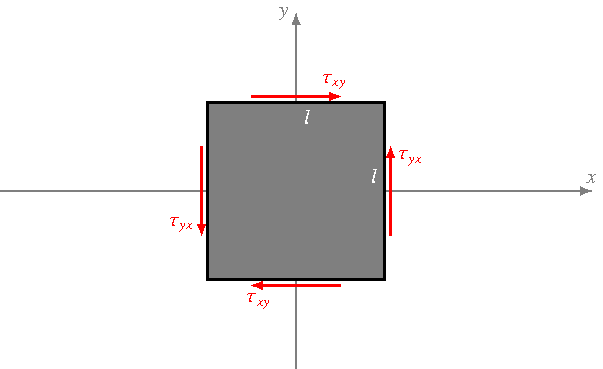
\includegraphics{chapters/2/drehmoment.pdf}
\caption{Drehmoment um die $z$-Achse der Schwerkräfte auf einen Würfel
mit Kantenlänge $2l$. Gezeigt sind nur die Komponenten von $\bm{\tau}$,
die zu einem Drehmoment führen.
\label{skript:drehmoment}}
\end{figure}
In diesem Abschnitt wollen wir nachweisen, dass der Spannungstensor
symmetrisch ist.
Dazu betrachten wir das Drehmoment, welches die Scherkräfte auf einen
kleinen Würfel mit Kantenlänge $2l$ ausüben (Abbildung \ref{skript:drehmoment}).

Der Würfel hat die Masse $m=\varrho(2l)^3$.
Das Trägheitsmoment eines Würfels mit Masse $m$ und Kantenlänge $2l$
ist
\[
I_z
=
\frac1{12}m((2l)^2+(2l)^2)
=
\frac1{12}\varrho 8l^3\cdot8l^2
=
\frac{16}{3}\varrho l^5.
\]
Der Drehimpuls um die $z$-Achse ist $L_z=I_z\omega$.

Aus Abbildung~\ref{skript:drehmoment} kann man die Scherkräfte auf den
Seitenflächen ablesen, sie sind $\tau_{xy}4l^2$ bzw.~$\tau_{yx}4l^2$,
ihr Hebelarm ist $l$.
Das resultierende Drehmoment um die $z$-Achse ist daher
\[
M_z = 8l^3\tau_{xy} - 8l^3\tau_{yx}.
\]
Die Bewegungsgleichungen eines starren Körpers besagen jetzt, dass
für die Winkelgeschwindigkeit der Drehung des Würfels um die $z$-Achse
die Gleichung
\[
\frac{dL_z}{dt}
=
M_z
\qquad\Rightarrow\qquad
I_z\dot\omega
=
M_z
\qquad\Rightarrow\qquad
\dot\omega
=
\frac{M_z}{I_z}
=
\frac{8l^3(\tau_{xy}-\tau_{yx})}{\frac{16}{3}l^5}
=
\frac{3}{2l^2}(\tau_{xy}-\tau_{yx}).
\]
Wir nehmen an, es sei $\tau_{xy}\ne\tau_{yx}$.
Lässt man $l$ gegen $0$ gehen, folgt die Aussage, dass die
Winkelgeschwindigkeit eines sehr kleinen Würfels im Fluid sich mit beliebig
schnell anwachsender Winkelgeschwindigkeit drehen müsste.
Dieses unphysikalische Resultat erlaubt zu schliessen, dass
$\tau_{xy}=\tau_{yx}$ sein muss und dass nur ein
symmetrischer Spannungstensor ein physikalisches Fluid beschreibt.

\subsubsection{Druck und Spannungen}
Die Diagonalelemente des Spannungstensors $\bm{\tau}$ beschreiben
Normalkräfte auf ein Volumenelement des Fluids.
Im Gleichgewicht sind sie alle gleich gross und stimmen mit dem
negativen {\em (hydrostatischen) Druck} überein, wir setzen daher
\index{Druck}
\index{hydrostatischer Druck}
\[
p=-\frac13\operatorname{Spur}\bm{\tau}.
\]
Wir können daher $\bm{\tau}$ zerlegen in eine Diagonalmatrix
mit Elementen $-p$ auf der Diagonalen und eine spurlose Matrix
\[
\bm{\tau} = -pE + \bm{\sigma},
\]
$E$ ist die Einheitsmatrix.
Die spurlose symmetrische Matrix $\bm{\sigma}$ heisst auch
{\em Spannungsdeviator}.
\index{Spannungsdeviator}

Für die Bewegungsgleichung brauchen wir die Divergenz beider Terme.
Die Druckterme sind alle gleich, nach
Definition~\ref{skript:definition divergenz} ist
\[
(\nabla\cdot(pE))_x
=
\sum_i
\frac{\partial p\delta_{xi}}{\partial i}
=
\frac{\partial p}{\partial x}
\qquad\Rightarrow\qquad
\nabla\cdot(pE)
=
\nabla p.
\]
Damit wird die Bewegungsgleichung 
\begin{equation}
\frac{\partial \varrho\vec{v}}{\partial t}
=
-\nabla\cdot(\varrho\vec{v}\vec{v})
+\varrho\vec b
-\nabla p
+\nabla\cdot\bm{\sigma}
\label{skript:navier-stokes2}
\end{equation}
Die Scherkräfte sind in einem newtonschen Fluid proportional zu
den Schergeschwindigkeiten.
Man kann zeigen (siehe \cite[p.~172]{skript:kaperengler}), dass $\bm{\sigma}$
geschrieben werden kann als
\[
\bm{\sigma}
=
2\nu\biggl(\bm{\varepsilon} - \frac13(\nabla\cdot\vec{v})E\biggr)
\qquad\text{mit}\qquad
\bm{\varepsilon}=\frac12\bigl(\nabla\vec{v}+(\nabla\vec{v})^t\bigr).
\]
Die spezielle Form von $\bm{\varepsilon}$ ist notwendig, damit die Matrix
$\bm{\varepsilon}$ symmetrisch wird.
Der zweite Term im Ausdruck für $\bm{\sigma}$ ist nötig, damit die Spur
\[
\operatorname{Spur}{\bm{\sigma}}
=
2\nu(\operatorname{\varepsilon} - \nabla\cdot\vec{v})
=
2\nu
\frac12
\biggl(
\sum_i \frac{\partial v_i}{\partial i}
+
\frac12
\sum_i \frac{\partial v_i}{\partial i}
-
\nabla\cdot\vec{v}
\biggr)
=
0
\]
von $\bm{\sigma}$ verschwindet.

Die Divergenz $\nabla\cdot\bm{\sigma}$ von $\bm{\sigma}$ kann damit explizit
durch die Geschwindigkeit ausgedrückt werden.
Wir berechnen die Divergenz der einzelnen Terme:
\begin{align}
(\nabla\cdot\bm{\varepsilon})_x
&=
\sum_i\frac{\partial \varepsilon_{ix}}{\partial i}
=
\frac12
\sum_i\frac{\partial}{\partial i}\biggl(
\frac{\partial v_i}{\partial x}+\frac{\partial v_x}{\partial i}
\biggr)
=
\frac{\partial}{\partial x}
\sum_i\frac{\partial v_i}{\partial i}
+
\frac12
\sum_i \frac{\partial^2 v_x}{\partial i^2}
=
\frac12\frac{\partial}{\partial x}
(\nabla\cdot\vec{v})
+
\frac12\Delta v_x
\notag
\\
\nabla\cdot\bm{\varepsilon}
&=
\frac12\nabla(\nabla\cdot\vec{v})
+
\frac12\Delta\vec{v}
\notag
\\
(\nabla\cdot(\nabla\cdot\vec{v})E)_x
&=
\sum_i \frac{\partial}{\partial i} (\nabla\cdot\vec{v}E)_{xi}
=
\sum_i \frac{\partial}{\partial i} (\nabla\cdot\vec{v}\delta_{xi})
=
\frac{\partial}{\partial x}(\nabla\cdot\vec{v})
\notag
\\
\nabla\cdot(\nabla\cdot\vec{v})E)
&=
\nabla(\nabla\cdot\vec v)
\notag
\\
\intertext{und erhalten so für die Divergenz von $\bm{\sigma}$:}
\nabla\cdot\bm{\sigma}
&=
2\nu\biggl(
\nabla\cdot\bm{\varepsilon}
-\frac13\nabla\cdot((\nabla\cdot\vec{v})E)
\biggr)
=
2\nu\biggl(
\frac12
\nabla(\nabla\cdot\vec{v})
+
\frac12\Delta\vec{v}
-\frac13
\nabla(\nabla\cdot\vec{v})
\biggr)
\\
&=
\nu\Delta\vec{v}
+\frac{\nu}3\nabla(\nabla\cdot\vec{v}).
\label{skript:sigmadiv}
\end{align}

\subsubsection{Inkompressible Strömung}
Da in einem inkompressiblen Fluid $\nabla\cdot\vec{v}=0$ ist, fällt
der zweite Term in \eqref{skript:sigmadiv} weg.
Die Strömungsgleichung eines inkompressiblen Fluids erhält damit die
einfache Form
\begin{equation}
\frac{\partial\vec{v}}{\partial t}
=
-\nabla\cdot(\vec{v}\vec{v})
+\vec{b}
-\frac1{\varrho}(\nabla p
-\nu\Delta\vec{v}),
\label{skript:inkompressibel newtonsch}
\end{equation}
die klassische Navier-Stokes Gleichung.
\index{Navier-Stokes Gleichung}%

\subsection{Zustandsgleichungen}
Die Dichte eines Gases hängt vor allem von der Temperatur und dem Druck ab.
In den Ozeanen ändert die Dichte des Wassers mit dem Salzgehalt.
Eine vollständige Beschreibung der Strömung in Ozeanen oder der
Atmosphäre muss daher auch noch weitere Variablen modellieren.
In Kapitel~\ref{chapter:wetter und klima} haben wir bereits auf die
Wärmeleitungsgleichungen hingewiesen.

Die Felder $T$, $p$ und $\varrho$ sind bei einem idealen Gas miteinander
durch die Zustandsgleichung
\[
p=\varrho T R_s
\]
mit der spezifischen Gaskonstante $R_s$ verbunden.
Für den Zusammenhang von Dichte, Temperatur und Salzgehalt gibt
es jedoch kein derart einfaches Modell.
Eine weitere Kopplung zwischen der Temperatur und der
Strömung entsteht durch die Viskosität $\nu$, die sehr stark
von der Temperatur abhängt.
Auch dafür gibt es keine einfachen Modelle.

In vielen Fällen schwanken die physikalischen Grössen nur geringfügig
um einen Mittelwert.
Zum Beispiel hängt die Dichte $\varrho$ von Meerwasser sowohl von
der Temperatur $T$ als auch vom Salzgehalt $S$ ab, die Dichte ist
also eine Funktion $\varrho(T,S)$.
Wir können $\varrho$ als Taylorreihe um die mittlere Temperatur $T_0$
und den mittleren Salzgehalt $S_0$ entwickeln:
\[
\varrho(T,S)
=
\varrho_0 -\alpha(T-T_0) + \beta(S-S_0).
\]
In Klimamodellen betrachten wir typischerweise nur kleine Abweichungen
von Mittelwerten, so dass ein solches Modell sehr erfolgreich sein kann.

\subsection{Boussinesq-Approximation}
Die Strömung in der Erdatmosphäre kann offensichtlich nicht als
inkompressibel betrachtet werden, die Dichte ist offenbar nicht
konstant.
Der Zustand der Atmosphäre weicht jedoch nur wenig einem mittleren
Dichteprofil $\varrho_0$ ab, welches im wesentlich durch das Temperaturprofil
festgelegt ist.
Im Normalzustand nimmt die Temperatur der Atmosphäre ziemlich genau
linear ab bis zur Höhe der Tropopause.
Auf die horizontale Komponente der Strömung hat eine Abweichung des
Temperaturprofils kaum einen Einfluss, denn andere Terme der
Navier-Stokes-Gleichung
\eqref{skript:navier-stokes2}
sind bedeutender.
Für die vertikale Bewegung ist der Term der äusseren Kräfte,
nämlich die Schwerkraft, dominant.
Wir können dies modellieren, indem wir die konstante Erdbeschleunigung
$g$ durch dichteabhängige Beschleunigung
\begin{equation}
g\frac{\varrho}{\varrho_0}
\label{skript:boussinesq}
\end{equation}
ersetzen.
Diese Approximation ist bekannt als die Boussinesq-Approximation.
Für unsere Zwecke brauchen wir nicht mehr als \eqref{skript:boussinesq}.
Dies wird bei der Herleitung der Lorenz-Gleichung in Abschnitt
\ref{section:lorenz-modell} benötigt.
Für die vollständigen Boussinesq-Gleichungen siehe \cite{skript:kaperengler}.

